\chapter{Estruturas}
\section{Custos}

Um levantamento orçamentário foi feito para a compra do material de construção do RaDop. Os custos aqui apresentados foram obtidos após contato com os fornecedores.

\begin{table}[h]
\resizebox{\textwidth}{!}{%
\begin{tabular}{|c|c|c|c|c|}
\hline
\multicolumn{5}{|c|}{Estrutura} \\ \hline
Quantidade & Material & Valor Unitário & Total & Fornecedor \\ \hline
2 & Caixa Para Painel Elétrico de Aço – 500x500x250 & R\$ 255,00 & R\$ 510,00 & Nobre Brasil \\ \hline
6 & Tubo Aço INOX 304 1m 2" 1.5mm & R\$ 41,00 & R\$ 246,00 & Fortinox \\ \hline
2 & Barra Chata 6m - 38,1x6,35mm & R\$ 53,59 & R\$ 107,18 & ArcelorMittal \\ \hline
2 & Abraçadeira União Horizontal Reforçada 3'' Kit Com 4 Peças & R\$ 52,90 & R\$ 105,80 & Mercado Livre \\ \hline
1 & Parafuso Sextavado M6 Aço Carbono Kit Com 100 Peças & R\$ 21,50 & R\$ 21,50 & Fortinox \\ \hline
1 & Rosca Sextavada M6 Aço Carbono Kit Com 100 Peças & R\$ 15,90 & R\$ 15,90 & Fortinox \\ \hline
1 & Ventilador para Painéis Elétricos Q110 & R\$ 180,00 & R\$ 180,00 & Vitória Ventiladores \\ \hline
1 & Eletroduto Zincado 1' 2m & R\$ 17,39 & R\$ 17,39 & Leroy Merlin \\ \hline
1 & Caixa Multipla 4x2 Com Rosca de Alumínio & R\$ 9,29 & R\$ 9,29 & Leroy Merlin \\ \hline
1 & Fio 2.5mm$^2$ 10m & R\$ 20,00 & R\$ 20,00 & Leroy Merlin \\ \hline
1 & Fio 4mm$^2$ 4m & R\$ 65,90 & R\$ 65,90 & Leroy Merlin \\ \hline
1 & Conduíte Corrugado 3/4 4m & R\$ 20,00 & R\$ 20,00 & Leroy Merlin \\ \hline
1 & Componentes Diversos & R\$ 100,00 & R\$ 100,00 & Leroy Merlin \\ \hline
TOTAL & - - & - - & R\$ 1.418,96 & - - \\ \hline
\end{tabular}%
}
\caption{Custos dos materiais para a estrutura}
\label{custosestruturas}
\end{table}

\section{Requisitos}

Os requisitos de Estruturas são:


\begin{itemize}
\item A estrutura deve suportar o peso de todos os componentes, com margem de segurança para eventuais cargas não estimadas;
\item Deve resistir à ação climática -- especificamente à radiação solar, temperatura elevada e corrosão devido à exposição à chuva;
\item A placa solar que fornecerá a energia do sistema deve ficar na parte lateral do conjunto, oposta à caixa de painel de controle superior;
\item Os sistemas de antena e câmera devem estar em montantes articulados à 3 metros de altura, para que a incidência possa ser ajustada e mais eficiente;
\item A estrutura deve permitir o acesso aos componentes de maneira facilitada, para descomplicar a manutenção do radar;
\item O vento incidente devido à região de instalação deve ser suportado pela estrutura.
\end{itemize}

\section{Restrições}
\begin{itemize}
\item Os materiais não podem ser suscetíveis à corrosão, à ruptura por radiação e temperatura solar;
\item Os compartimentos de instalação dos eletrônicos não podem permitir a entrada de água ou detritos externos;
\item Os compartimentos não podem estar totalmente isolados, permitindo acesso para reparos e manutenção;
\item Os materiais selecionados não podem impedir o funcionamento de qualquer um dos componentes eletrônicos.
\end{itemize}

\section{Riscos}

\begin{itemize}
\item RSN 1 - Atrasos no fornecimento de materiais;
\item RSN 2 - Montagem mal feita;
\item RSN 3 - Interferência da estrutura nos equipamentos de radiofrequência;
\item RSN 4 - Atrasos causados por problemas de simulações e modelagem;
\item RSN 5 - Curto circuito de componentes eletrônicos causados pela estrutura;
\item RSN 6 - Dimensionamento errado;
\item RSN 7 - Fatores climáticos extremos.
\end{itemize}

\section{Solução Proposta}

A estrutura visa a acomodação dos componentes eletrônicos de forma segura e possibilitando a manutenção de forma ágil, quando necessário. Estudos sobre a fiação, esforços, tensões e dissipação de calor foram feitos para a construção de uma estrutura que cumpra seu papel sem falhas.

\section{Materiais Utilizados}

Foi definido para o projeto a utilização de caixas de painel de controle, pois essas atendem todas as necessidades do projeto. A construção das caixas não era viável por conta da falta de maquinário necessário, além do fato de que caixas comerciais são mais leves e resistentes. Elas também possuem um preço mais acessível do que a compra de chapas de aço para usinar e contruí-las. As caixas são de aço e possuem 1 mm de espessura, com dimensões de 500x500x250 mm. São rígidas e resistentes à corrosão, com tratamento de fosfato de zinco e pintura a pó. Ambas possuem borrachas de vedação hermética e possuem grau de proteção IP54 conforme a ABNT NBR IEC 60529 \cite{material}. 

Duas hastes de aço inox 304 com 2 polegadas de diâmetro (50,80 mm) serão utilizadas para suportar todos os módulos necessários da estrutura. Essas medidas foram selecionadas com base nos cálculos numéricos feitos para medir os esforços e tensões a que elas serão submetidas (esse cálculos serão apresentados neste relatório). As hastes também foram selecionadas com base nas suas propriedades de rigidez e resistência à corrosão. O fator comercial também foi algo decisivo na escolha do material. Cada haste terá 4 metros, porém foi definido a utilização de 1 metro para que a estrutura fosse enterrada já que a fixação ou a criação de um fundação não será possível na fase de implementação do projeto. 

\subsection{Desenho Industrial}

Utilizou-se o software CATIA V5 para a criação do CAD (\textit{computer aided design}) da estrutura. A estrutura completa, apresentado na Figura \ref{estrucomp} foi construída com base nas medidas das caixas comerciais e hastes selecionadas. Além disso, as medidas também foram pensadas para terem uma proporção com os painéis solares. 

\begin{figure}[h]
	\centering
    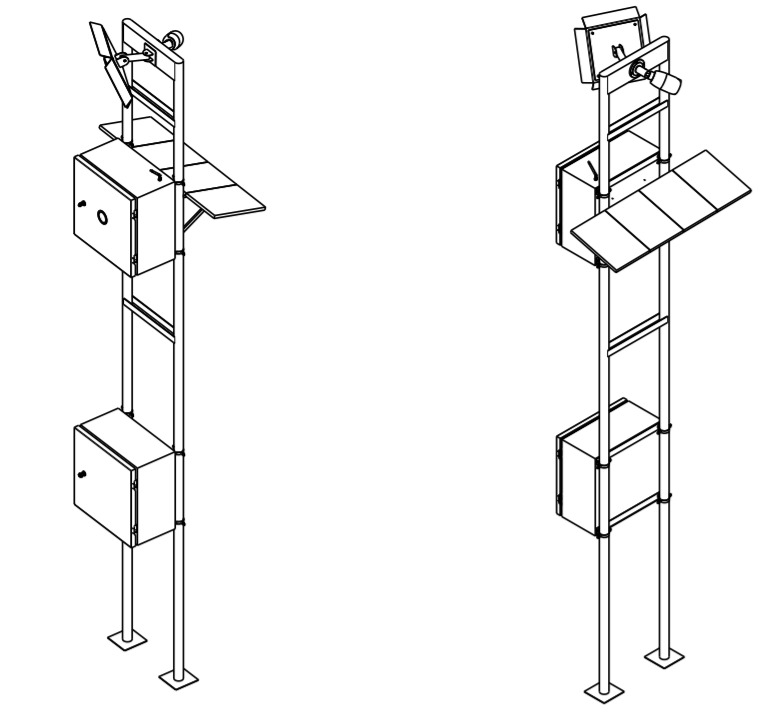
\includegraphics[scale=0.3]{estruturacompleta.jpeg}
    \caption{Design completo da estrutura com todos os seus módulos instalados.}
    \label{estrucomp}
\end{figure}


Na Figura \ref{hastes}, vemos o suporte principal. Ele consiste em dois tubos de aço afastados entre si a uma distancia de 450 mm. Seu desenvolvimento foi pensado de forma a garantir a estabilidade da estrutura. Por isso é possível ver a utilização de barras chatas de aço soldadas nas hastes para que o sistema seja mais rígido.

\begin{figure}[h]
	\centering
    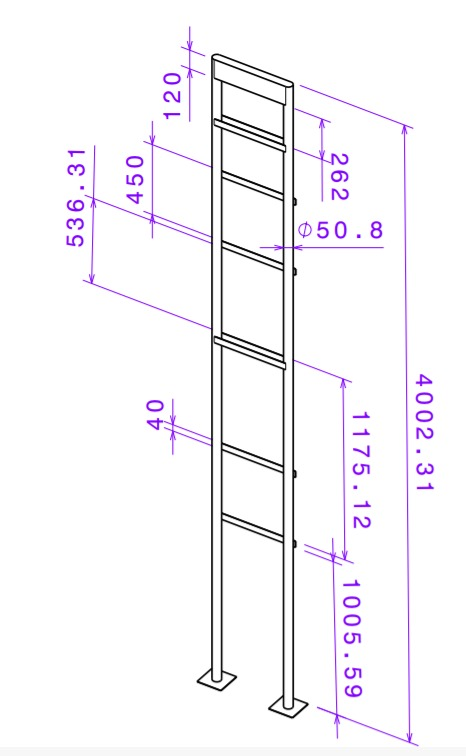
\includegraphics[scale=0.3]{hastes.jpeg}
    \caption{Hastes de suporte para acoplar os módulos da estrutura com cotas.}
    \label{hastes}
\end{figure}

A caixa inferior, apresentada na Figura \ref{caixainf}, será apoiada no chão, pois a mesma carregará a bateria do sistema. Por questões técnicas, se a mesma ficasse na caixa superior com os componentes eletrônicos poderia aquecê-los a uma temperatura que causaria o mal funcionamento do sistema por completo. A caixa inferior estará ligada através de 4 abraçadeiras do tipo união às hastes de suporte principal.

\begin{figure}[h]
	\centering
    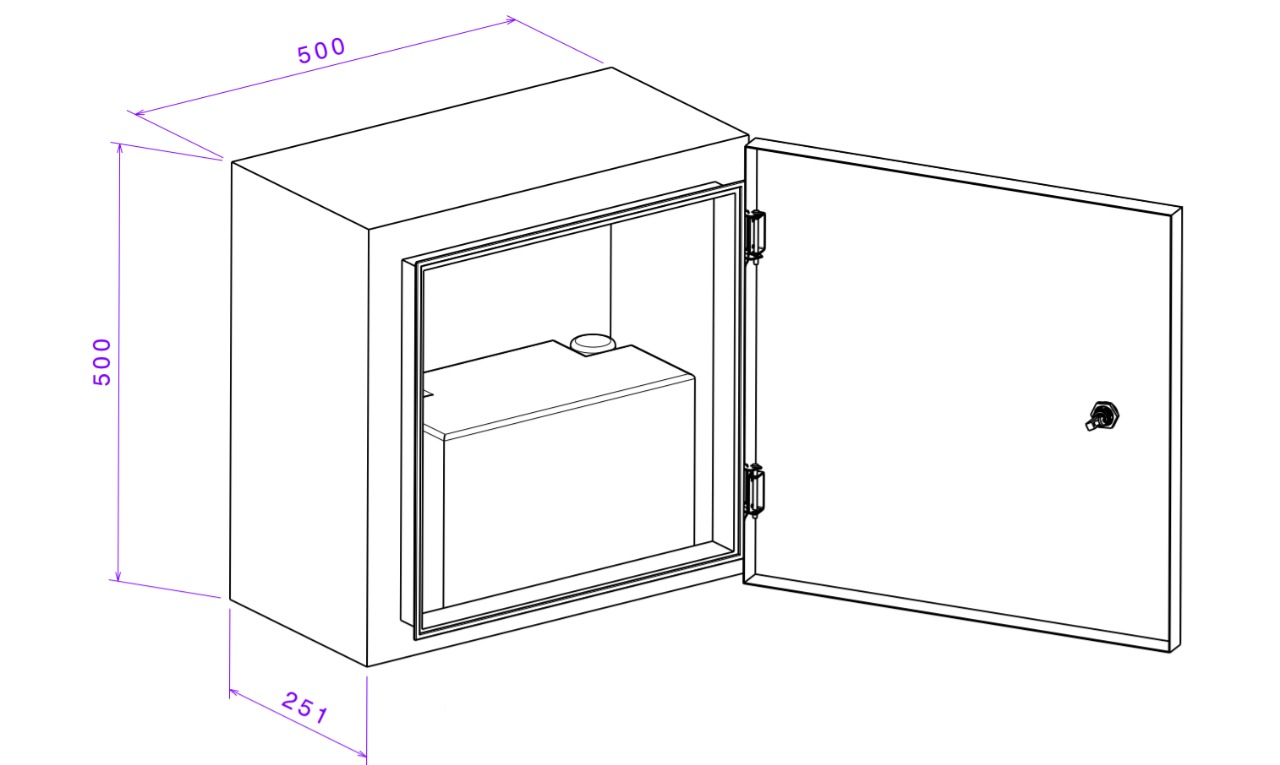
\includegraphics[scale=0.3]{caixainferior.jpeg}
    \caption{Caixa inferior aberta com bateria acoplada e seu isolamento hermético.}
    \label{caixainf}
\end{figure}

A caixa superior, apresentado na Figura \ref{caixasup}, será o local onde os componentes eletrônicos ficarão. Todo o transporte de informações acontecerá nela. Os componentes vão possuir um espaço de 300x300mm em uma placa de montagem para seus devidos acoplamentos. Um \textit{cooler} será instalado na lateral interna da caixa superior para ajudar na dissipação do calor. 

\begin{figure}[h]
	\centering
    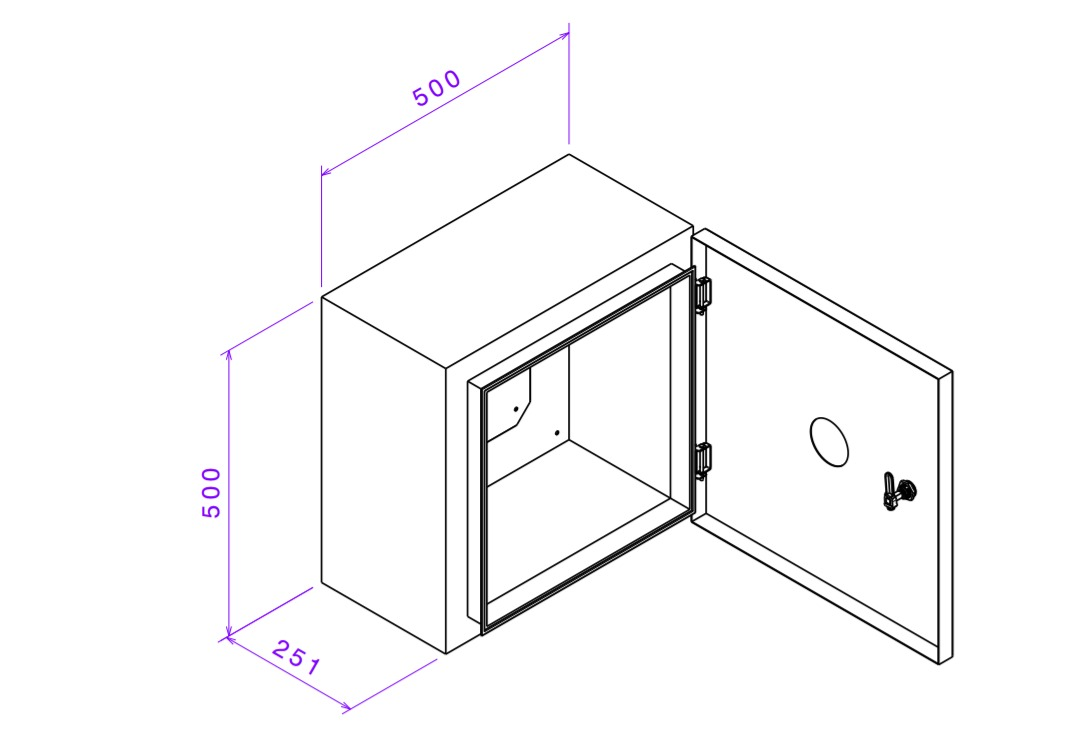
\includegraphics[scale=0.3]{caixasuperior.jpeg}
    \caption{Caixa inferior aberta com furo na porta para o holofote, placa de montagem e seu isolamento hermético.}
    \label{caixasup}
\end{figure}

Em sua porta será fixado um holofote, apresentado na Figura \ref{holof}, que servirá de sinal luminoso para o motorista. Ambas as caixas possuem trancas com chaves para evitar a abertura acidental ou por pessoa não autorizada.

\begin{figure}[h]
	\centering
    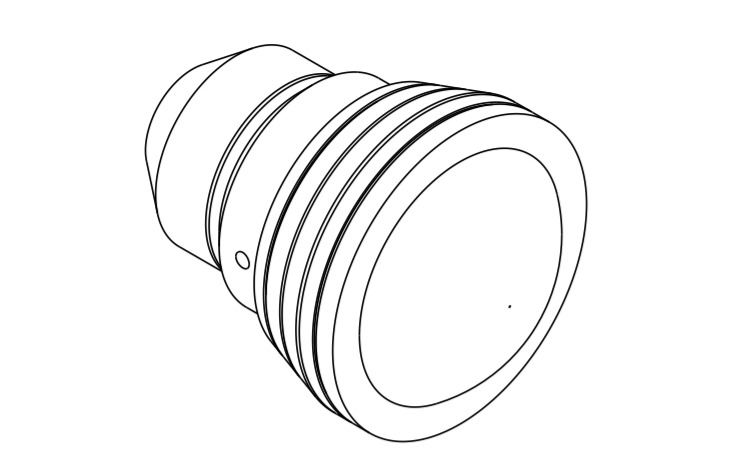
\includegraphics[scale=0.3]{holofote.jpeg}
    \caption{Modelo do holofote comercial que servirá de sinal luminoso ao motorista.}
    \label{holof}
\end{figure}

O painel solar, apresentado na Figura \ref{painelsol}, se encontra logo atrás da caixa superior. Será necessário a construção de um suporte para o mesmo e será soldado às hastes em 4 ponto,s com uma angulação de 15 graus conforme solicitado pela equipe do projeto responsável pela área de energia. 

\begin{figure}[h]
	\centering
    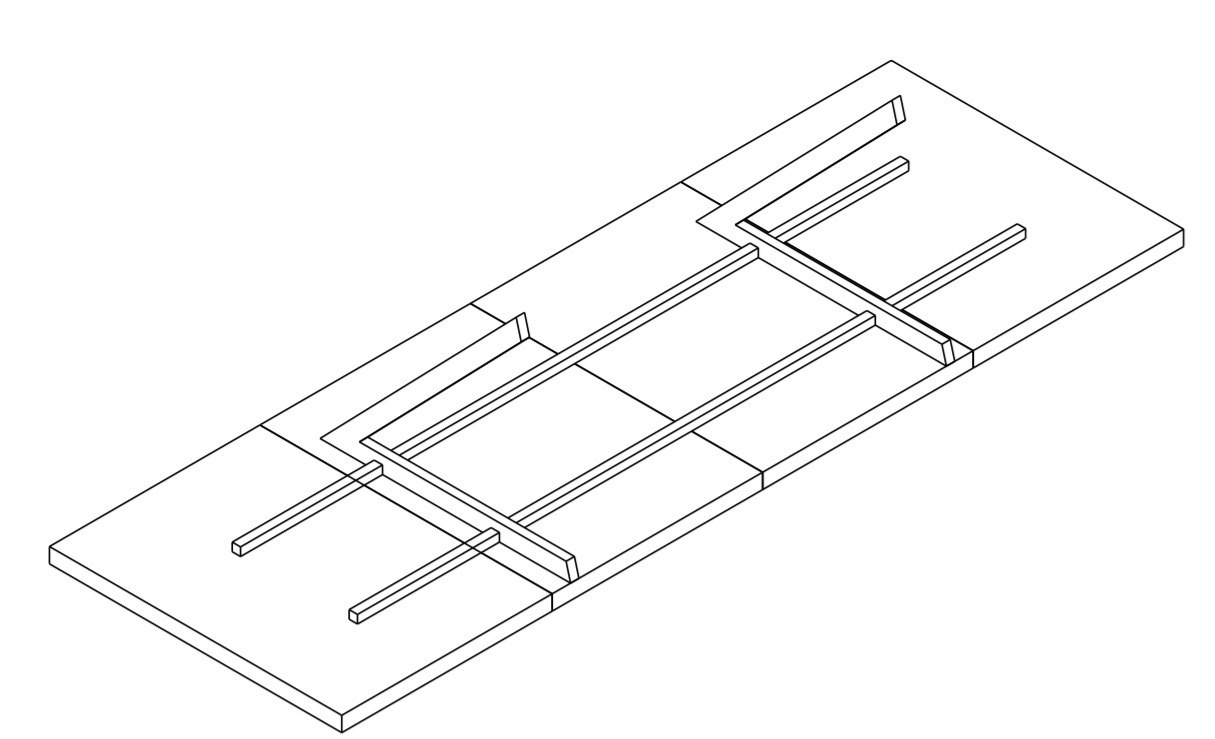
\includegraphics[scale=0.3]{painelcomsup.jpeg}
    \caption{Painel solar com suporte que será soldado às hastes da estrutura.}
    \label{painelsol}
\end{figure}

No ponto mais alto da estrutura, a 3 metros do chão, teremos dois componentes. A antena do radar \textit{Doppler} e a câmera. A câmera, apresentado na Figura \ref{camera}, possui apenas um grau de liberdade. Sendo assim, é necessário o acoplamento dela de forma correta para garantir a angulação necessária para capturar com eficiência as imagens dos carros. 

\begin{figure}[h]
	\centering
    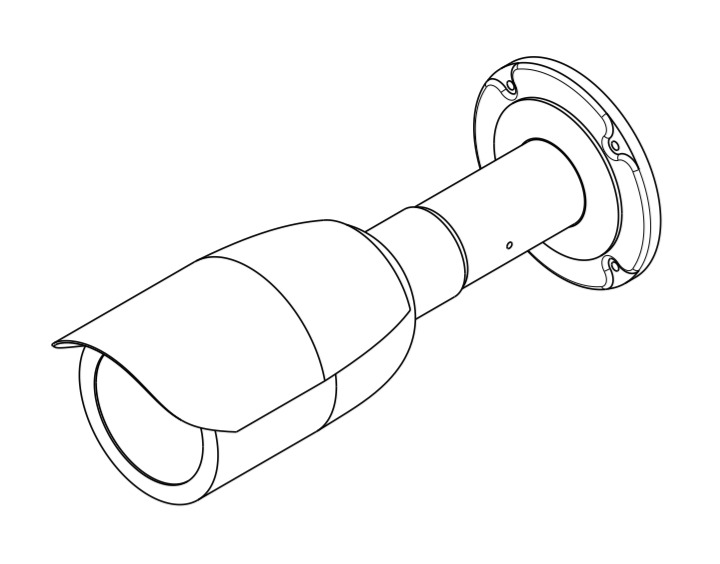
\includegraphics[scale=0.3]{camera.jpeg}
    \caption{Modelo da câmera comercial para capturar a placa veicular.}
    \label{camera}
\end{figure}

Oposta à câmera, teremos a antena do radar \textit{Doppler}, apresentada na Figura \ref{antrad}. Ela possuirá um suporte que dará a ela dois graus de liberdade, possibilitando assim uma facilidade no ajuste necessário para uma maior eficiência. 

\begin{figure}[h]
	\centering
    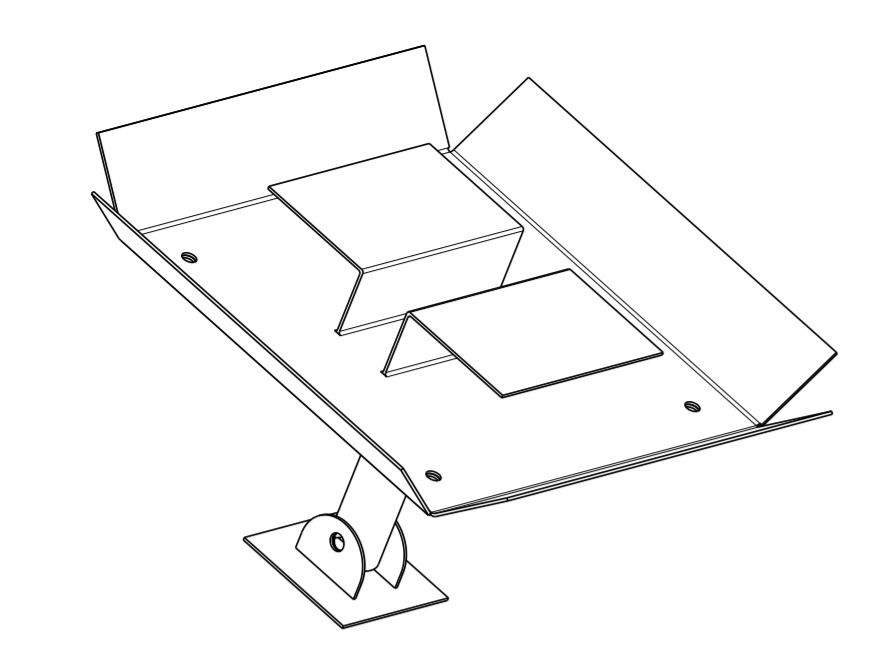
\includegraphics[scale=0.3]{antenaradar.jpeg}
    \caption{Antena para o radar \textit{Doppler}.}
    \label{antrad}
\end{figure}

As plantas detalhadas, com cotas, para a construção de todas as peças se encontram no Apêndice \ref{plantas_construcao}. 

\subsection{Diagrama de Fiação}

Para o dimensionamento da parte elétrica, foi utilizada a NBR 5410 \cite{protecao} para instalações elétricas em circuitos de extra baixa tensão, apresentado na Figura \ref{circ}. A equipe de estruturas foi responsável por posicionar a fiação na estrutura. 

\begin{figure}[h]
	\centering
    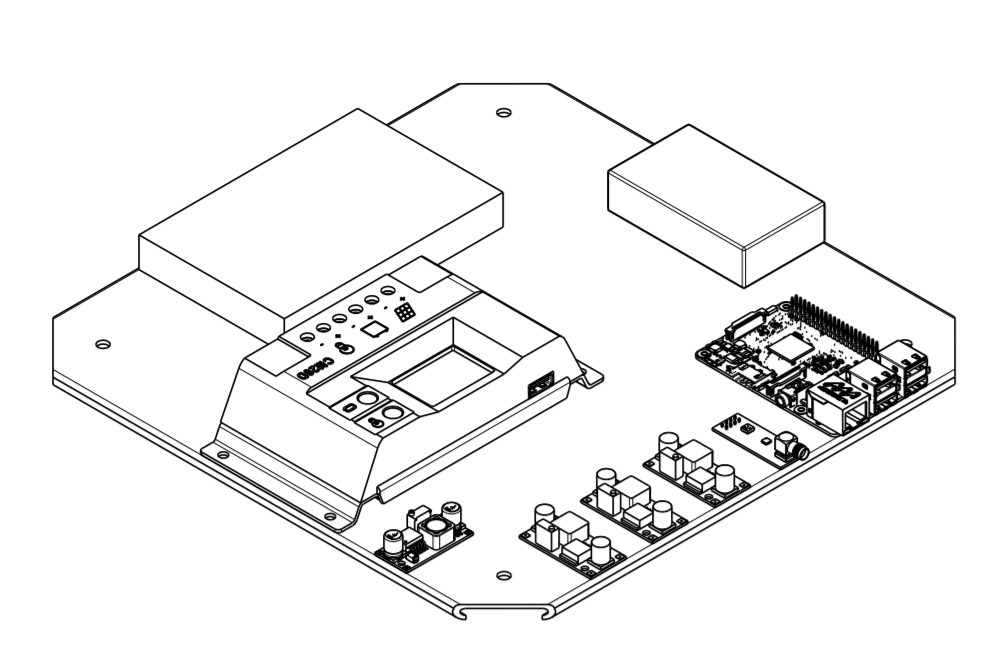
\includegraphics[scale=0.3]{placademontagemcomcomp.jpeg}
    \caption{Placa de montagem da caixa superior com componentes eletrônicos instalados.}
    \label{circ}
\end{figure}


Como os componentes eletrônicos ficarão em compartimentos suspensos por abraçadeiras, a solução mais robusta e viável seria a utilização de eletrodutos, apresentado na Figura \ref{eletrod}, instalados nas colunas de sustentação comunicando os dois compartimentos (da bateria e do Nuand + Raspberry Pi 3+) e conectando os compartimentos aos instrumentos (radar, câmera, painel solar e holofote).

\begin{figure}[h]
	\centering
    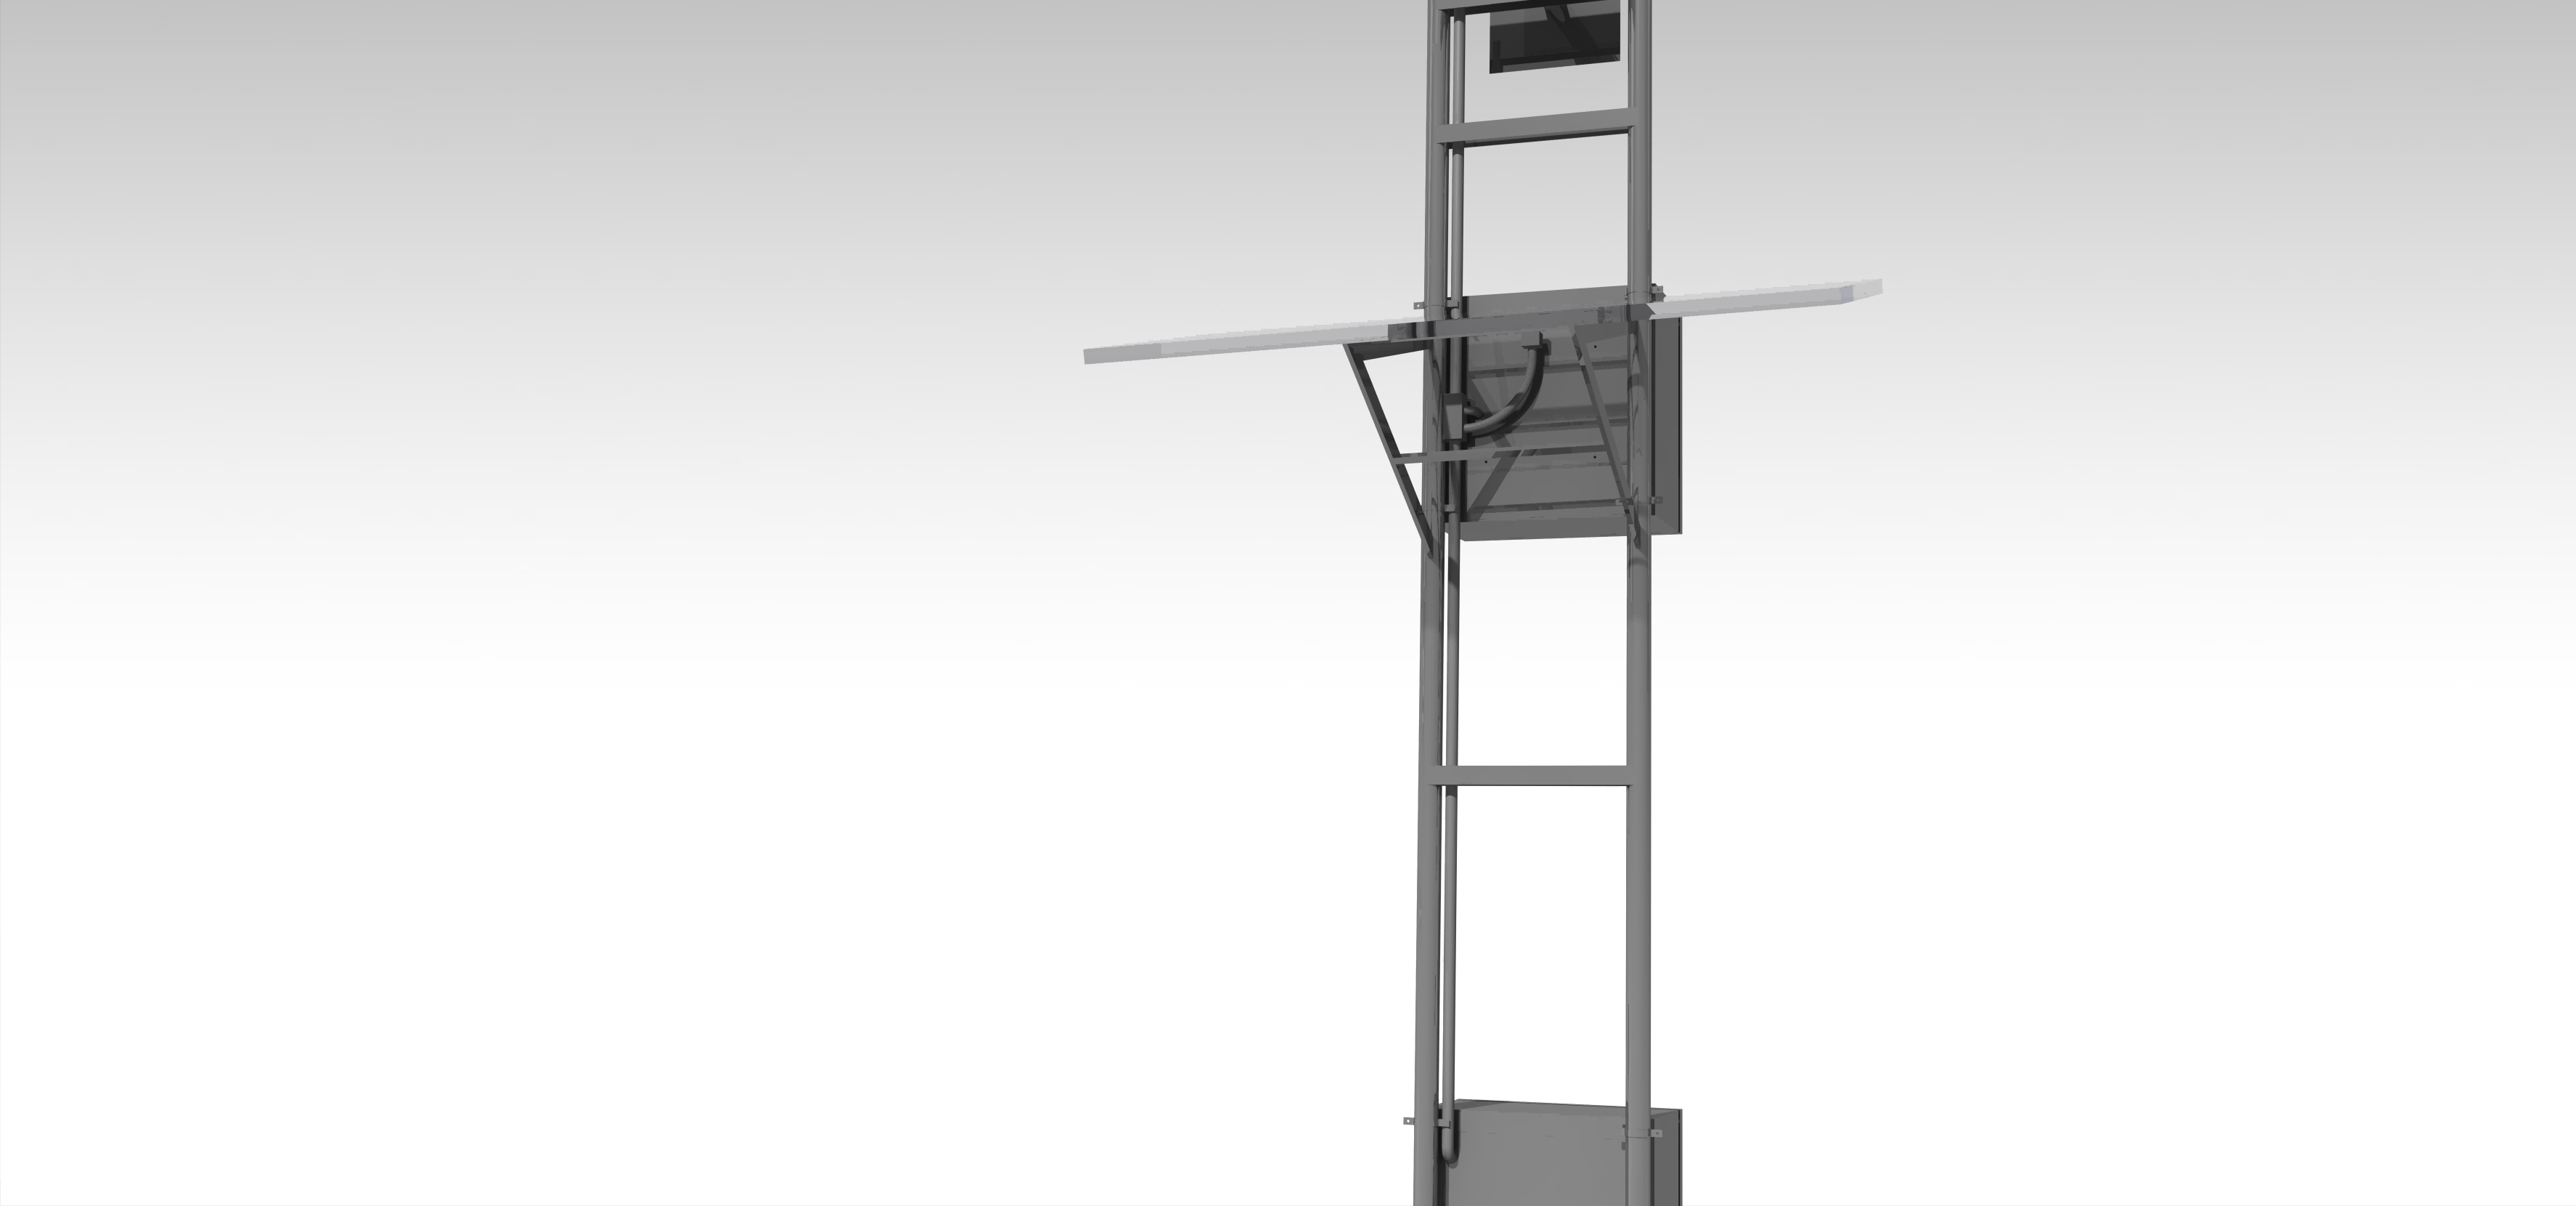
\includegraphics[scale=0.5]{eletrodutos.png}
    \caption{Disposição dos eletrodutos na estrutura conectando as caixas superior e inferior, o radar, o painel solar e a câmera.}
    \label{eletrod}
\end{figure}

Disposição dos eletrodutos:

\begin{itemize}
\item 1 eletroduto conectando o compartimento inferior a uma caixa de distribuição (eletroduto galvanizado);
\item 1 eletroduto galvanizado da caixa de distribuição superior para o radar e a câmera;
\item 1 eletroduto flexível saindo da caixa de distribuição superior para o painel solar.
\end{itemize}

Como os circuitos utilizados são de extrema baixa tensão, a NBR-5410 \cite{protecao} diz que a seção mínima dos fios devem ser de 0,7mm$^2$, entretanto a equipe utilizou fios de 2,5mm$^2$ nos fios por terem uma maior resistência estrutural e facilitar a manutenção, como apresentado na Figura \ref{caixa1elet}.

\begin{figure}[h]
	\centering
    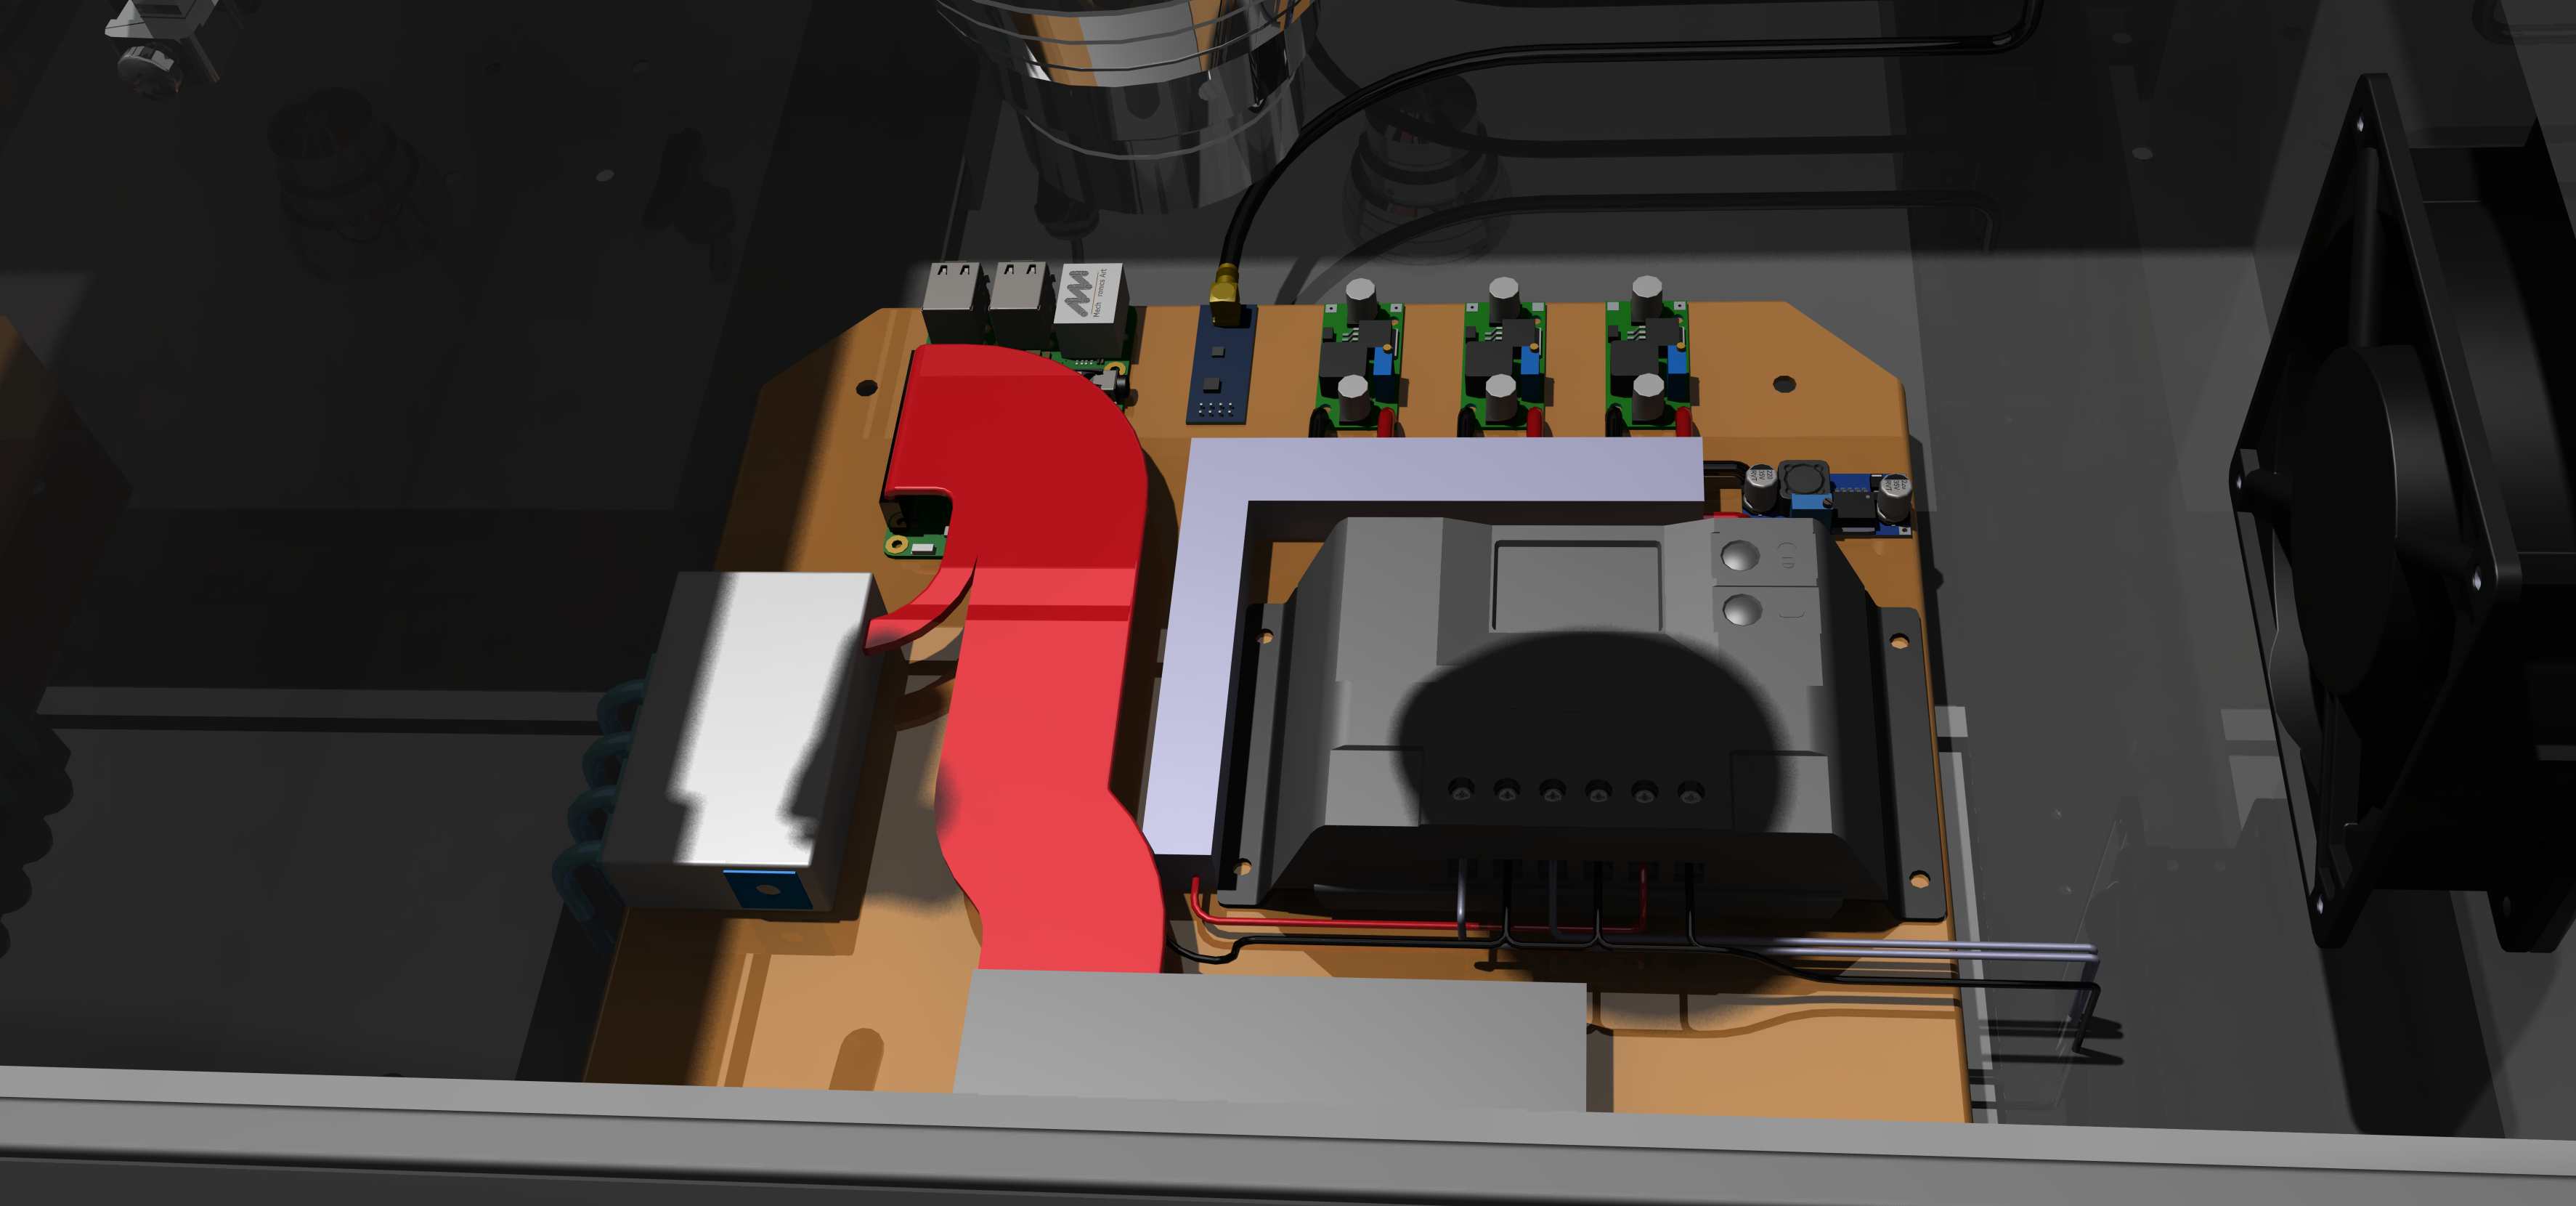
\includegraphics[keepaspectratio=true,scale=0.5]{caixa1elet.png}
    \caption{Disposição do dimensionamento da fiação dos dispositivos eletrônicos dentro da caixa superior.}
    \label{caixa1elet}
\end{figure}


 Na bateria, a fiação escolhida foi de 35mm$^2$ pois foi utilizado nos cálculos a corrente de descarga nominal da bateria. Entretanto a fiação da bateria sairá do compartimento inferior, como apresentado na Figura \ref{caixa2elet}.

\begin{figure}[h]
	\centering
    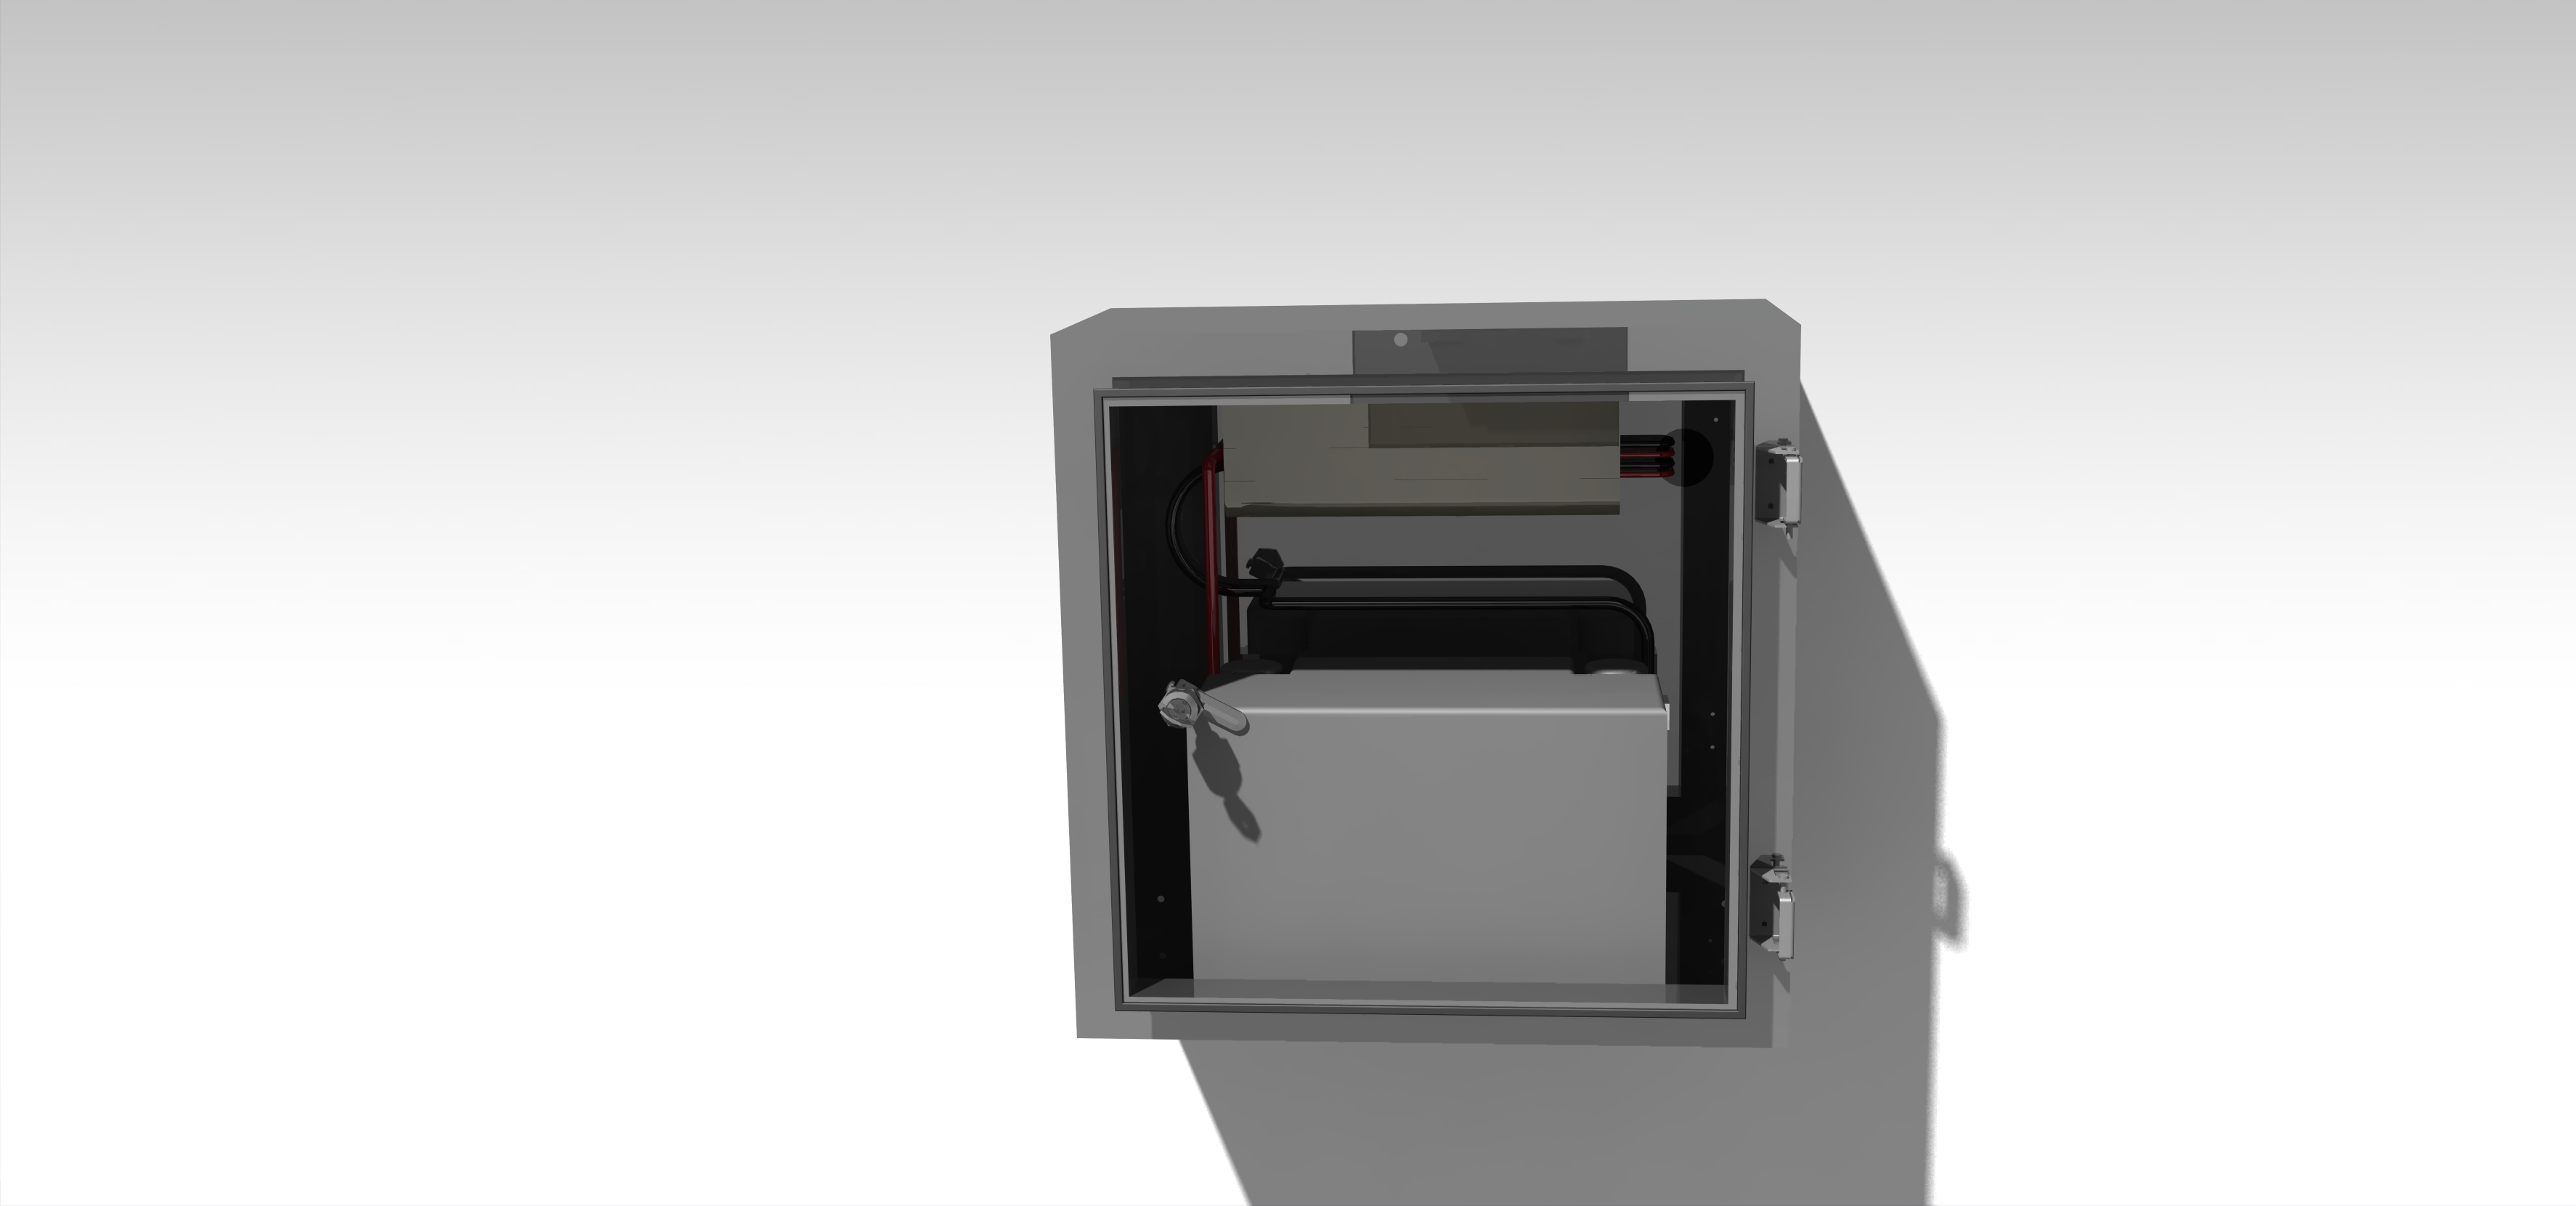
\includegraphics[scale=0.5]{caixa2elet.png}
    \caption{Disposição do dimensionamento da fiação dos dispositivos eletrônicos dentro da caixa inferior com a bateria.}
    \label{caixa2elet}
\end{figure}



\subsection{Análise Estática da Estrutura}

Para o cálculo estrutural, foi desenvolvida uma rotina em MATLAB que fornecesse o diâmetro das hastes em relação às tensões normais e cisalhantes nas mesmas de acordo com as propriedades mecânicas dos materiais selecionados (Apêndice \ref{codigo_estatico}).


A força dinâmica causada pela força do vento foi calculada segundo a norma NBR 6123 (jun/88) \cite{vento} e foram aplicadas à estrutura como cargas pontuais e constantes. O valor do vento para o projeto, também retirado da norma, é de 6m/s.

Os materiais prévios considerados para o trabalho eram aços (inox 304, 1010, 1020, 1030 e 1045) e ferro. O ferro foi um material considerado para o projeto pois possui um peso específico menor que o do aço, porém possui as propriedades mecânicas mais restritas. Percebeu-se que seria necessário mais material para poder chegar às mesmas condições que os aços, e por isso foi desconsiderado. As propriedades dos aços são bem parecidas, mudando as tensões de escoamento e tensão última (propriedades principais para o projeto).

Para a modelagem do problema foi considerado uma estrutura simétrica, e a tensão admissível pelos componentes estruturais é a tensão de escoamento do aço levando em consideração um fator de segurança. O material usado para o cálculo foi o aço inox 304 com a tensão de escoamento no valor de 215 MPa \cite{callister}. Estimando o peso de cada componente em Catia e utilizando a metodologia para os cálculos de tensão principais \cite{beer}, foi possível determinar os esforços na estrutura.

A rotina ((Apêndice \ref{codigo_estatico}), considerou um apoio de engaste e calculou os esforços externos que a estrutura está submetida (esforços normais, cortantes e momento). Sendo os esforços normais causados pelo peso dos componentes acoplados às hastes de sustentação e o peso das próprias hastes, e os esforços cortantes causados pelo efeitos dinâmicos sofridos por causa do vento. O momento é a força gerada pelo braço de alavanca entre essas forças e as suas respectivas distâncias ao chão.


A força dinâmica causada pela força do vento foi calculada segundo a norma NBR 6123 (jun/88) \cite{vento} e foram aplicadas à estrutura como cargas pontuais e constantes, o valor do vento para o projeto, também retirado da norma, é de 6m/s.	

O diâmetro mínimo gerado pela rotina foi de aproximadamente 0,05m (2 polegadas). Pelo o projeto contar com duas hastes estruturais, o valor do diâmetro encontrado é suficiente para as cargas aplicadas. A escolha do diâmetro, também se dá em função da facilidade comercial. Foram feitos levantamentos em 5 lojas sendo que os padrões de diâmetro variam apenas em números inteiros.

Analisando a estrutura em Ansys, foi possível a obtenção das tensões equivalente de \textit{Von-Mises} e o deslocamento da estrutura, sendo esta máxima em 14.56mm.

A Figura \ref{fig:maximo} apresenta o local de esforço máximo e o comportamento da tensão nas presilhas que suportam as caixas.

\begin{figure}[h]
	\centering
    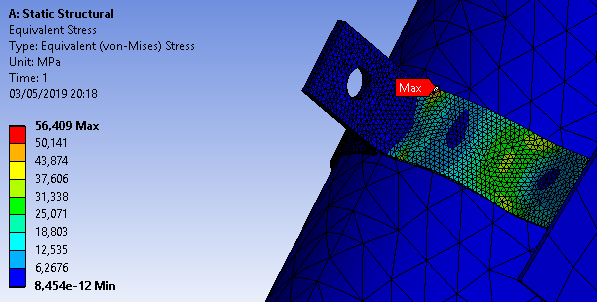
\includegraphics[scale=0.7]{max_tension}
    \caption{Tensão equivalente de \textit{Von-Mises} para as presilhas.}
    \label{fig:maximo}
\end{figure}

A Figura \ref{fig:base}, apresenta o local de esforço máximo e o comportamento da tensão base da estrutura.

\begin{figure}[h]
	\centering
    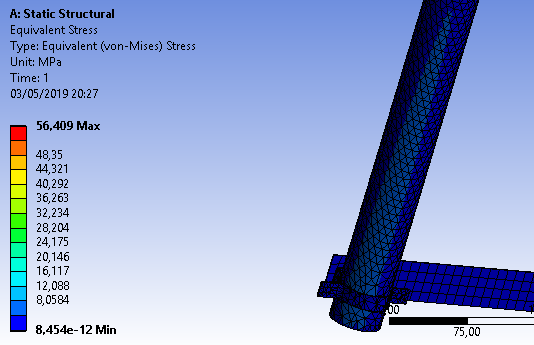
\includegraphics[scale=0.7]{base_tension}
    \caption{Tensão equivalente de \textit{Von-Mises} na base.}
    \label{fig:base}
\end{figure}

A Figura \ref{fig:painel}, apresenta o local de esforço máximo e o comportamento da tensão no suporte para o painel solar.

\begin{figure}[h]
	\centering
    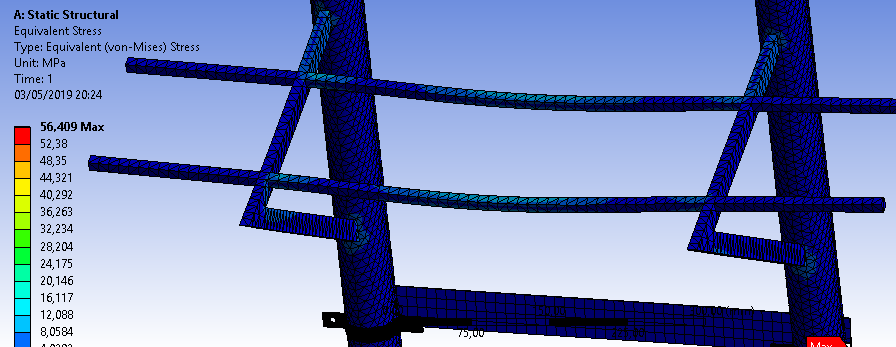
\includegraphics[scale=0.6]{painel_tension}
    \caption{Tensão equivalente de \textit{Von-Mises} para o suporte para o painel solar.}
    \label{fig:painel}
\end{figure}

%\section{Análise Dinâmica da Estrutura}

\section{Estudo da Dissipação de Calor na Estrutura}

Devido ao fato da escolha do material para a estrutura ser metálico e o Brasil ter abundância em incidência solar, deve-se garantir que a temperatura de operação estará entre 20 e $30\%$ abaixo da temperatura limite dos componentes \cite{temperatura}. Tendo em vista que a temperatura limite de operação é 50$^{\circ}C$, a temperatura de operação foi fixada em 36$^{\circ}C$. Para modelagem do problema é proposto um ventilador elétrico, para a indução de dissipação por convecção combinada (natural e forçada) e dissipador de calor no processador da \textit{Raspberry}, devido à sua maior temperatura de operação.

Para o dimensionamento do ventilador, foi inicialmente considerado em regime permanente, a 1 atm, o ar sendo um gás ideal e a radiação negligenciável, tendo em vista que é um ambiente fechado.

A Figura \ref{cooler}, mostra um esquemático do comportamento do fluxo de ar em torno de uma placa plana, quando quente, gerando um fluxo de ar forçado devido ao ventilador e quando frio um refluxo contrário ao ventilador gerando um efeito de convecção natural \cite{livro_transcal}.

\begin{figure}[h]
	\centering
    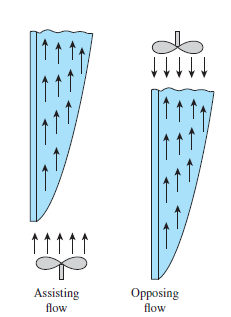
\includegraphics[keepaspectratio=true,scale=0.5]{cooler.png}
    \caption{Esquemático do fluxo de ar devido ao ventilador \cite{livro_transcal}.}
    \label{cooler}
\end{figure}

Desta forma, com uma rotina em Matlab (Apêndice \ref{codigo_dissipacao}), definindo a temperatura nas superfícies da caixa como 60$^{\circ}C$, as propriedades do ar no ambiente da caixa como a média entre a temperatura de operação e a de superfície, e a partir de uma vazão do ventilador média de 25$m^3/h$, visto em catálogo, o número de Reynolds e Grashof são determinados. 

A Eq. \ref{reynolds}, descreve o cálculo para o número de Reynolds, para o comportamento forçado do escoamento, onde $v$ é a velocidade do ventilador, estimada a partir da vazão, $L_c$ é o comprimento característico de interesse, e $\upsilon$ é a viscosidade dinâmica do ar.

\begin{equation}
	Re= \frac{v \times L_c}{\upsilon}.
	\label{reynolds}
\end{equation}

A Eq. \ref{grashof}, descreve o cálculo para o número de Grashof, para o comportamento natural do escoamento, onde $g$ é a gravidade, $\beta$ é o inverso da temperatura média em Kelvin, $T_S$ é a temperatura na superfície e $T_{\infty}$ é a temperatura ambiente desejada.

\begin{equation}
	Gr= \frac{g \beta (T_S-T_{\infty})L_c^3}{\upsilon^2}.
	\label{grashof}
\end{equation}

A eficiência entre o escoamento natural (Grashof) sobre o quadrado do escoamento forçado (Reynolds), da qual o número de Nusselt correto (natural, forçado ou combinado) para a definição da potência dissipada, considerando parede vertical ou horizontal \cite{livro_transcal}. Tendo o Nusselt, determina-se o coeficiente de transferência de calor de convecção $h$ e a potência dissipada pela Eq. \ref{potencia}.

\begin{equation}
	\dot{Q}= hA_s(T_S-T_{\infty}).
	\label{potencia}
\end{equation}

Onde $\dot{Q}$ é a dissipação de calor e $A_s$ é a área da superfície de interesse. Após feito os cálculos a dissipação se ver predominante na região horizontal, por isso o ventilador fica de lado aos componentes, com uma dissipação na ordem de $40W$.

Para a determinação do tempo necessário para se alcançar o regime permanente, foi modelado como um sistema aglomerado, no qual é avaliado a resistência a condução do corpo em relação a resistência a convecção, o número de Biot e a taxa de condução de calor do corpo em relação a taxa de armazenamento de calor, o número de Fourier \cite{livro_transcal}. Fazendo uma proximação unidimensional do problema, o tempo estimado é de cerca de 1h. Por ser um tempo considerável, foi-se definido que o ventilador ficaria durante todo o período do dia ligado.


Por ser uma modelagem aproximada, e pela dificuldade computacional de simulação serão realizados testes com a caixa para a validação do modelo. 

